\documentclass[tikz,border=2pt]{standalone}
\usepackage{amsmath,amssymb}
\usepackage{pgfplots}
\pgfplotsset{compat=1.18}

\begin{document}
% Conditioning Y ~ Exp(2) on the event A = {Y > 1}: keep the density on A and divide by
% P(A) = e^{-2}; the result 2e^{-2(y-1)} is the same shape restarted at 1.
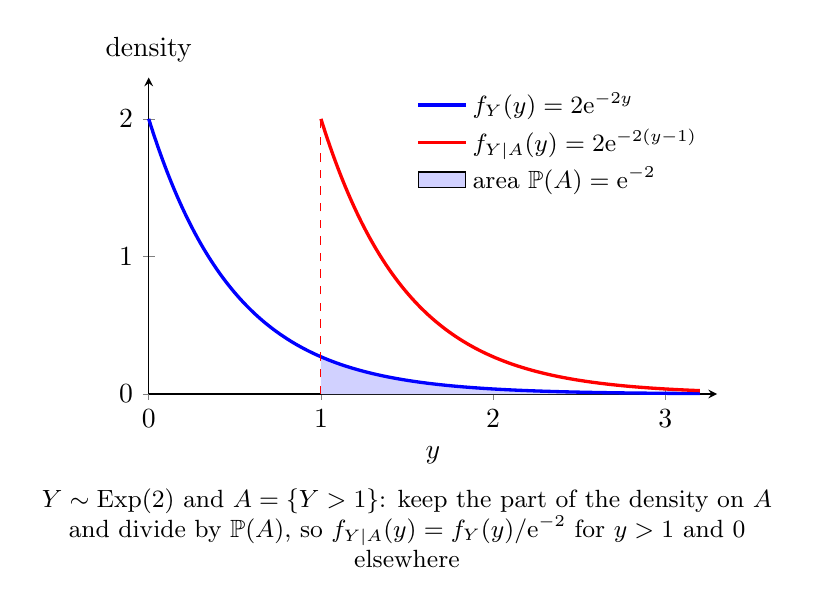
\begin{tikzpicture}
	\begin{axis}[
		axis lines=left, xmin=0, xmax=3.3, ymin=0, ymax=2.3,
		xtick={0,1,2,3}, ytick={0,1,2},
		xlabel={$y$}, ylabel={density}, ylabel style={rotate=-90, anchor=south, at={(axis description cs:0,1.02)}},
		samples=120, smooth, width=8.8cm, height=5.6cm, clip=false,
		legend style={draw=none, fill=none, font=\small, at={(0.99,0.99)}, anchor=north east}, legend cell align=left
		]
		\addplot[fill=blue!18, draw=none, domain=1:3.2, forget plot] {2*exp(-2*x)} \closedcycle;
		\addplot[blue, very thick, domain=0:3.2] {2*exp(-2*x)};
		\addlegendentry{$f_Y(y)=2\mathrm{e}^{-2y}$}
		\addplot[red, very thick, domain=1:3.2] {2*exp(-2*(x-1))};
		\addlegendentry{$f_{Y\mid A}(y)=2\mathrm{e}^{-2(y-1)}$}
		\addlegendimage{area legend, fill=blue!18, draw=none}
		\addlegendentry{area $\mathbb{P}(A)=\mathrm{e}^{-2}$}
		\draw[red, dashed] (axis cs:1,0) -- (axis cs:1,2);
	\end{axis}
	\node[anchor=north, font=\small, align=flush center, text width=9.4cm] at ([yshift=-2pt]current axis.outer south) {$Y\sim\operatorname{Exp}(2)$ and $A=\{Y>1\}$: keep the part of the density on $A$ and divide by $\mathbb{P}(A)$, so $f_{Y\mid A}(y)=f_Y(y)/\mathrm{e}^{-2}$ for $y>1$ and $0$ elsewhere};
\end{tikzpicture}
\end{document}
